\chapter{LaTeX testing stuff}
\label{LaTeX testing stuff}
LaTeX testing stuff...
\rule{2.6cm}{0.75pt}  \hspace{3cm} üü \rule{3cm}{0.75pt}\\[2cm]
\begin{itemize}
	\item LaTeX testing stuff
	\item LaTeX testing stuff LaTeX testing stuff
\end{itemize}


\section{Section name}
\begin{enumerate}
	\item Siia midagi nummerdatut
	\item veel midagi
\end{enumerate}
\subsection{subsection name}


\begin{minted}{c}
int main() {
printf("hello, world");
return 0;
}
\end{minted}
\begin{minted}{sh}
echo $(pidof mysql)
apt-get install firefox
$333
\end{minted}
\inputminted{sh}{code/simple.sh}

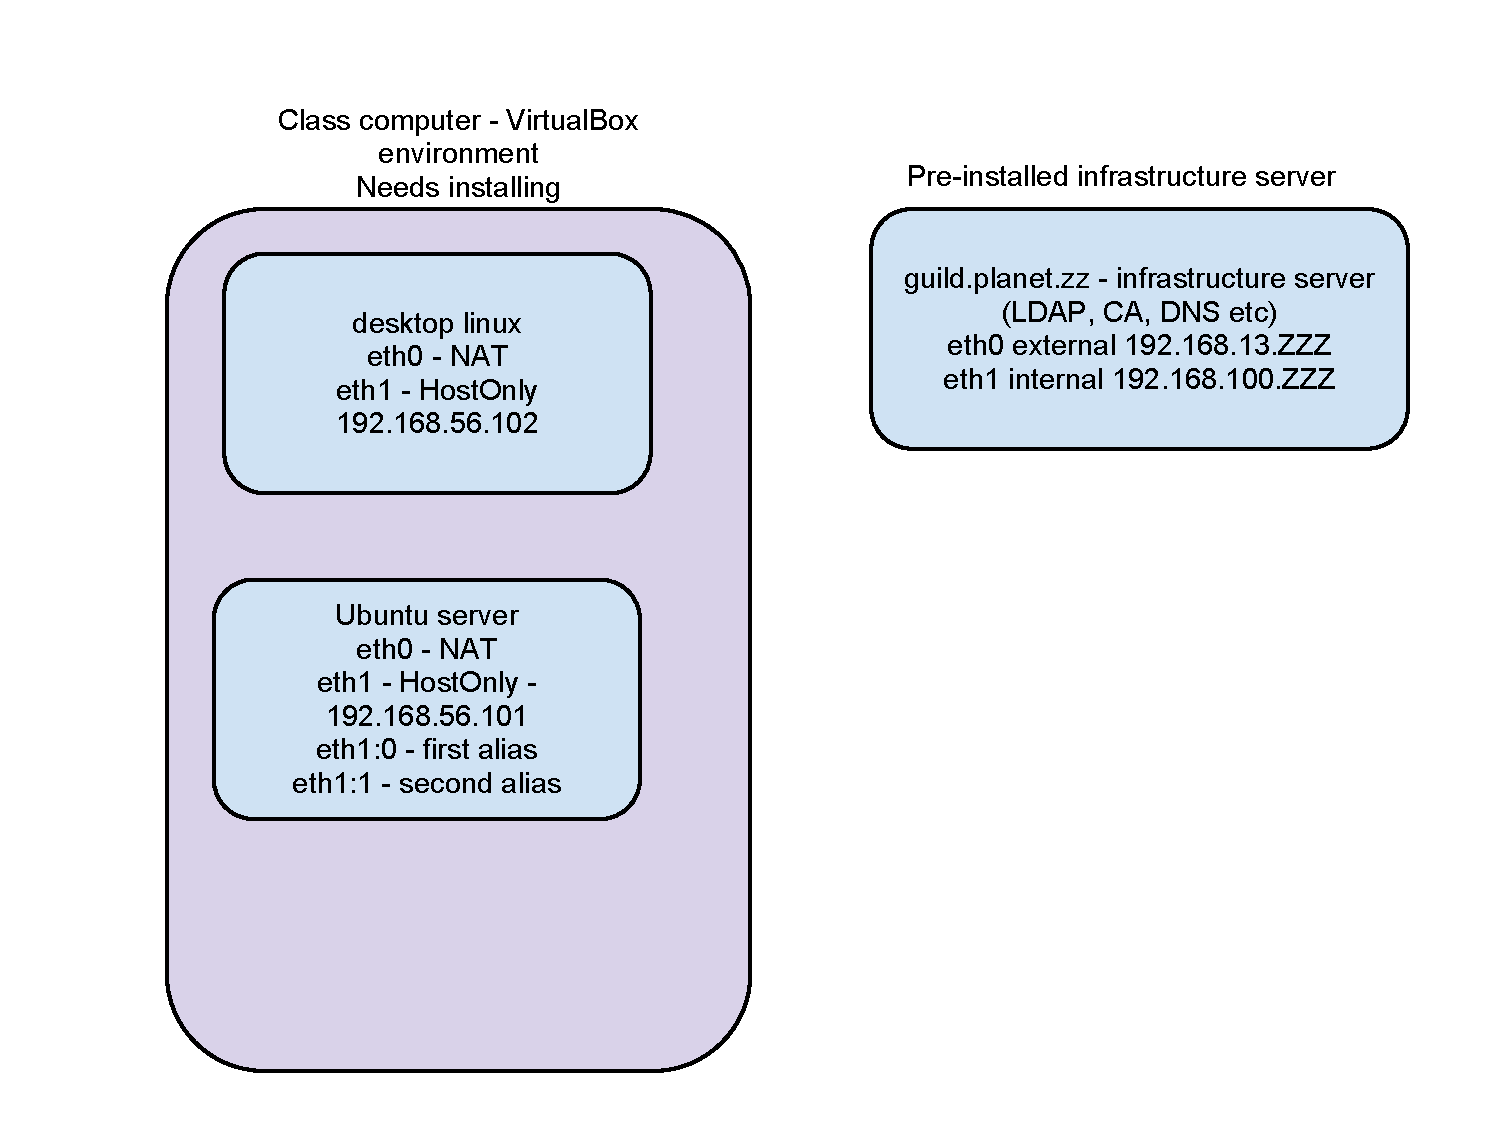
\includegraphics[width=\textwidth]{Lab_setup.pdf}
dddddd d  e d dwe \

\mint{ruby}|puts "hello world in ruby"|\

\cite{website:ssl} Bla bla
\citep{book:code-complete} d  d
\citep{OppeArenduskeskus2010} de dede
\cite{url:pulse} ewd wed
\citep{SecEngineering} wewde
